\documentclass[11pt]{article}
\usepackage{amsmath, amssymb, physics, mathtools, bm}
\usepackage{tikz, pgfplots}
\pgfplotsset{compat=1.18}
\usepackage[margin=2.3cm]{geometry}
\usepackage{siunitx, booktabs, hyperref}
\usepackage{braket}

\newcommand{\D}{\mathrm{D}}
\newcommand{\de}{\mathrm{d}}
\newcommand{\pd}[2]{\frac{\partial #1}{\partial #2}}
\newcommand{\pdd}[2]{\frac{\partial^{2} #1}{\partial #2^{2}}}
\newcommand{\Lap}{\nabla^{2}}

\title{B6 Condensed-Matter Physics --- Model Solutions, 2018}
\author{}
\date{}

\begin{document}
\maketitle

\section*{Question 1 --- Crystal structure of tungsten}

\textbf{Problem.} Identify lattice types of $\alpha$- and $\beta$-tungsten; from the lowest-angle powder XRD ring of $\alpha$-W (\SI{0.1542}{nm} X-rays, $2\theta=40.26^\circ$) deduce $a$ and the density; for $\beta$-W find the first two non-vanishing rings, their intensity ratio, and the lowest-angle additional weak ring expected.

\subsection*{(a) Definition and lattice type of $\alpha$-W}

A \emph{lattice} is the infinite set of points
\[
\bm R = n_1\bm a_1 + n_2\bm a_2 + n_3\bm a_3,\qquad n_i\in\mathbb Z,
\]
generated by three primitive vectors $\bm a_i$; every lattice point has identical environment.

For $\alpha$-W, the two atoms at $[0,0,0]$ and $[\tfrac12,\tfrac12,\tfrac12]$ are chemically identical and have identical local environments, so each is a lattice point. The conventional cubic cell with the centring vector $[\tfrac12,\tfrac12,\tfrac12]$ is
\[
\boxed{\;\text{body-centred cubic (BCC).}\;}
\]

\subsection*{(b) Lattice constant and density}

Selection rule (BCC): reflections allowed for $h+k+l$ even; lowest-$\sin\theta$ ring is $(110)$.

Bragg's law:
\[
\lambda = 2 d_{110}\sin\theta.
\]
Solve for $d_{110}$:
\[
d_{110} = \frac{\lambda}{2\sin\theta} = \frac{\SI{0.1542}{nm}}{2\sin(20.13^\circ)}.
\]
Evaluate denominator: $2\sin(20.13^\circ) = 0.6884$:
\[
d_{110} = \SI{0.2240}{nm}.
\]
Cubic spacing $d_{hkl}=a/\sqrt{h^2+k^2+l^2}$:
\[
a = d_{110}\sqrt{2}.
\]
Numerical:
\[
\boxed{\;a = \SI{0.3168}{nm}.\;}
\]

BCC conventional cell contains 2 atoms. Mass density:
\[
\rho = \frac{2 M}{N_A a^3}.
\]
Insert numbers:
\[
\rho = \frac{2 \times \SI{0.1838}{kg\,mol^{-1}}}{(\SI{6.022e23}{mol^{-1}})\,(\SI{3.168e-10}{m})^3}.
\]
Evaluate $a^3$: $a^3 = \SI{3.179e-29}{m^3}$:
\[
\rho = \frac{\SI{0.3676}{kg\,mol^{-1}}}{\SI{1.914e-5}{m^3\,mol^{-1}}}.
\]
Final:
\[
\boxed{\;\rho \approx \SI{1.92e4}{kg\,m^{-3}} = \SI{19.2}{g\,cm^{-3}}.\;}
\]

\subsection*{(c) Lattice type of $\beta$-W}

The two corner/centre atoms $\{[0,0,0],[\tfrac12,\tfrac12,\tfrac12]\}$ have a different local environment from the six face-pair atoms $[\tfrac14,\tfrac12,0]$ etc., so the eight sites are \emph{not} all equivalent: they cannot all be lattice points.

Test BCC centring $\bm T=[\tfrac12,\tfrac12,\tfrac12]$:
\[
[\tfrac14,\tfrac12,0] + [\tfrac12,\tfrac12,\tfrac12] = [\tfrac34,1,\tfrac12]\equiv [\tfrac34,0,\tfrac12],
\]
which is not in the basis: BCC ruled out. FCC and primitive face centring similarly fail. Hence
\[
\boxed{\;\text{simple (primitive) cubic, with an 8-atom basis (A15 structure).}\;}
\]

\subsection*{(d) First two rings of $\beta$-W and their intensity ratio}

All eight atoms have the same form factor $f$. Structure factor:
\[
S_{hkl} = f\sum_{j=1}^{8} e^{2\pi i(h x_j + k y_j + l z_j)}.
\]
Group corner/centre pair $\times$ face-pair triplet:
\[
S_{hkl} = f\bigl[1+(-1)^{h+k+l}\bigr]\Bigl\{1 + 2\cos\tfrac{\pi h}{2}\cos\pi k + 2\cos\tfrac{\pi l}{2}\cos\pi h + 2\cos\tfrac{\pi k}{2}\cos\pi l\Bigr\}.
\]
First bracket vanishes for $h+k+l$ odd: $(100),(110),(111)$ absent.

Tabulate $|S/f|^2$ and multiplicity $m$:
\begin{center}
\begin{tabular}{cccc}
\toprule
$(hkl)$ & $h^2+k^2+l^2$ & $|S/f|^2$ & $m$ \\
\midrule
(200) & 4 & 16 & 6 \\
(210) & 5 & 16 & 24 \\
(211) & 6 & 16 & 24 \\
(220) & 8 & 0 & --- \\
\bottomrule
\end{tabular}
\end{center}

First two non-vanishing rings:
\[
\boxed{\;(200)\ \text{and}\ (210).\;}
\]

Both have $|S|^2 = 16 f^2$, so the ratio is set by multiplicity (Lorentz-polarisation and Debye-Waller corrections are subleading):
\[
\frac{I_{210}}{I_{200}} \approx \frac{m_{210}}{m_{200}} = \frac{24}{6}.
\]
\[
\boxed{\;\frac{I_{210}}{I_{200}} \approx 4.\;}
\]

\subsection*{(e) Additional weak ring at lower angle}

The cancellations producing $|S|=0$ for $h+k+l$ odd assumed all 8 sites have identical scattering. The two Wyckoff sites are chemically inequivalent: corner/centre atoms vibrate differently from face-pair atoms, giving distinct anisotropic Debye--Waller factors and slightly different effective form factors, $f_1\neq f_2$.

With $f_1\neq f_2$ the structure factor becomes $S = (f_1-f_2)\times[\text{previously-vanishing prefactor}]$, so previously forbidden rings reappear with intensity $\propto (f_1-f_2)^2 \ll (f_1+f_2)^2$.

Lowest forbidden ring (smallest $h^2+k^2+l^2$): $(100)$. However $(100)$ also vanishes from the second bracket on the corner/centre sublattice; the lowest ring with non-zero contrast between the two sublattices is
\[
\boxed{\;(110),\;}
\]
seen weakly because $|f_1-f_2|\ll f$.

\section*{Question 2 --- Tight binding}

\textbf{Problem.} Define $\mu$ and $E_F$. For a 1D tight-binding chain with hopping $-t$, derive the dispersion, sketch it and the DOS. For monovalent atoms find $E_F$ and show $\mu(T)=E_F$. Repeat the Fermi-surface and $\mu(T)$ analysis on a 2D square lattice, then on a squeezed rectangular lattice.

\subsection*{(a) Definitions}

Chemical potential: $\mu = \left(\partial U/\partial N\right)_{S,V}$, the energy cost of adding one particle at fixed entropy and volume; equivalently, the energy at which the Fermi--Dirac function equals $\tfrac12$.

Fermi energy: $E_F = \mu(T=0)$, the energy of the highest occupied single-particle state in the ground state of a non-interacting fermion system.

\subsection*{(b) 1D dispersion, BZ diagram, DOS}

Expand a single-particle eigenstate $\ket{\psi}=\sum_n \psi_n\ket{n}$. Apply $H$:
\[
H\ket{\psi} = \sum_n \psi_n\bigl(\epsilon_0\ket{n} - t\ket{n+1} - t\ket{n-1}\bigr).
\]
Project onto $\bra{m}$:
\[
E\,\psi_m = \epsilon_0\,\psi_m - t\,\psi_{m-1} - t\,\psi_{m+1}.
\]
Bloch ansatz $\psi_n = e^{ikna}$:
\[
E = \epsilon_0 - t\,e^{-ika} - t\,e^{ika}.
\]
Combine exponentials:
\[
\boxed{\;E(k) = \epsilon_0 - 2t\cos(ka),\qquad k\in(-\pi/a,\pi/a].\;}
\label{eq:tb1d}
\]

DOS in 1D follows from $g(E)\,\de E = (L/\pi)\de k$ (factor 2 for spin already absorbed by per-atom counting):
\[
g(E) = \frac{L}{\pi}\frac{1}{|\de E/\de k|} = \frac{L}{\pi a}\frac{1}{\sqrt{(2t)^2 - (E-\epsilon_0)^2}}.
\]
Van Hove singularities at $E=\epsilon_0\pm 2t$.

\begin{center}
\begin{tikzpicture}[>=stealth, scale=1.1]
  % Dispersion plot
  \draw[->] (-3.2,0) -- (3.2,0) node[right] {$k$};
  \draw[->] (0,-1.6) -- (0,1.6) node[above] {$E(k)-\epsilon_0$};
  \draw[domain=-3:3, smooth, variable=\x, thick, blue]
    plot ({\x}, {-1.2*cos(deg(\x*pi/3))});
  \node[circle,fill,inner sep=1.2pt] at (-3,1.2) {};
  \node[circle,fill,inner sep=1.2pt] at ( 3,1.2) {};
  \node[circle,fill,inner sep=1.2pt] at (0,-1.2) {};
  \node[left] at (-3,0) {$-\pi/a$};
  \node[right] at (3,0) {$\pi/a$};
  \node[right] at (0,1.2) {$+2t$};
  \node[right] at (0,-1.2) {$-2t$};
\end{tikzpicture}
\hspace{0.6cm}
\begin{tikzpicture}[>=stealth, scale=1.1]
  % DOS sketch
  \draw[->] (-2.8,0) -- (2.8,0) node[right] {$E-\epsilon_0$};
  \draw[->] (0,0) -- (0,2.2) node[above] {$g(E)$};
  \draw[domain=-1.95:1.95, smooth, samples=120, variable=\x, thick, blue]
    plot ({\x}, {0.6/sqrt(4 - \x*\x)});
  \node[circle,fill,inner sep=1.2pt] at (-2,0) {};
  \node[circle,fill,inner sep=1.2pt] at ( 2,0) {};
  \node[below] at (-2,0) {$-2t$};
  \node[below] at ( 2,0) {$+2t$};
\end{tikzpicture}
\end{center}

\subsection*{(c) Half-filling: $E_F$ and $\mu(T)$}

Bandwidth $4t$, $N$ atoms, $2N$ spin states, $N$ electrons (monovalent): half-filled. Symmetry $E(k+\pi/a)-\epsilon_0 = -[E(k)-\epsilon_0]$ gives $g(\epsilon_0+\delta)=g(\epsilon_0-\delta)$.

At $T=0$, fill the lower half of the band:
\[
\boxed{\;E_F = \epsilon_0.\;}
\]

Particle number constraint at any $T$:
\[
N_e = \int g(E)\,n_F(E,\mu,T)\,\de E = \tfrac12\int g(E)\,\de E.
\]
Apply hint $n_F(E,\mu) = 1 - n_F(2\mu - E,\mu)$:
\[
\int g(E)\,n_F(E,\mu)\,\de E = \int g(E)\,\de E - \int g(E)\,n_F(2\mu - E,\mu)\,\de E.
\]
Substitute $E\to 2\mu - E$ in the second integral, with $g(2\mu-E)$ appearing:
\[
\tfrac12\int g(E)\,\de E = \int g(E)\,\de E - \int g(2\mu-E)\,n_F(E,\mu)\,\de E.
\]
Demand consistency with $g(2\epsilon_0 - E) = g(E)$: the equation collapses to an identity iff $\mu=\epsilon_0$:
\[
\boxed{\;\mu(T) = \epsilon_0 = E_F\quad\text{for all }T.\;}
\]
Particle--hole symmetry pins $\mu$ to the band centre.

\subsection*{(d) 2D square lattice, monovalent}

Brillouin zone: square $-\pi/a < k_x,k_y \le \pi/a$. Half-filling sets $\cos(k_x a) + \cos(k_y a) = 0$: a square rotated by $45^\circ$, vertices $(\pm\pi/a,0),(0,\pm\pi/a)$.

\begin{center}
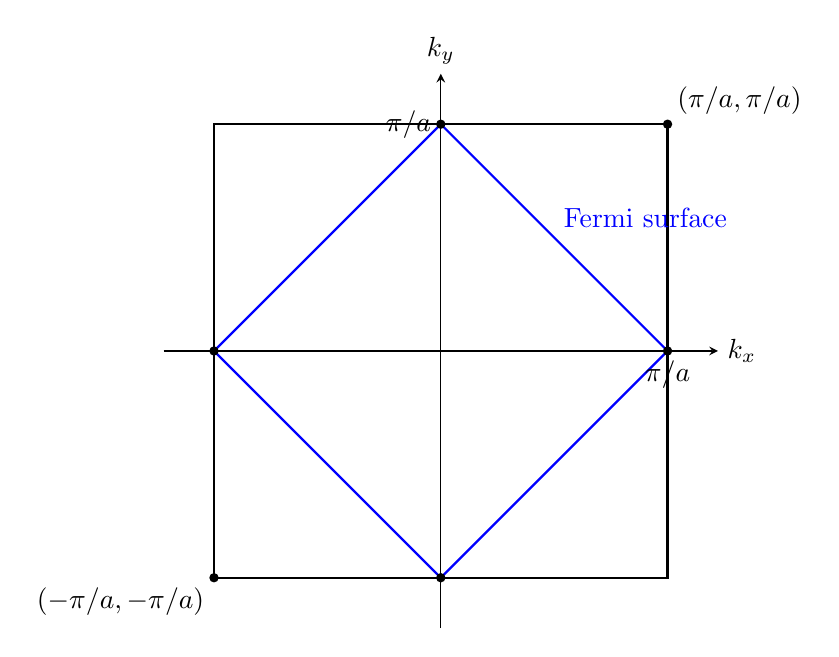
\begin{tikzpicture}[>=stealth, scale=1.6]
  \draw[->] (-2.2,0) -- (2.2,0) node[right] {$k_x$};
  \draw[->] (0,-2.2) -- (0,2.2) node[above] {$k_y$};
  \draw[thick] (-1.8,-1.8) rectangle (1.8,1.8);
  \draw[thick, blue] (-1.8,0) -- (0,1.8) -- (1.8,0) -- (0,-1.8) -- cycle;
  \node[circle,fill,inner sep=1.2pt] at ( 1.8,0) {};
  \node[circle,fill,inner sep=1.2pt] at (-1.8,0) {};
  \node[circle,fill,inner sep=1.2pt] at (0, 1.8) {};
  \node[circle,fill,inner sep=1.2pt] at (0,-1.8) {};
  \node[circle,fill,inner sep=1.2pt] at ( 1.8, 1.8) {};
  \node[circle,fill,inner sep=1.2pt] at (-1.8,-1.8) {};
  \node[above right] at ( 1.8, 1.8) {$(\pi/a,\pi/a)$};
  \node[below left]  at (-1.8,-1.8) {$(-\pi/a,-\pi/a)$};
  \node[below] at ( 1.8,0) {$\pi/a$};
  \node[left]  at (0, 1.8) {$\pi/a$};
  \node[blue, above right] at (0.9,0.9) {Fermi surface};
\end{tikzpicture}
\end{center}

Nesting $E(\bm k+\bm Q)+E(\bm k) = 2\epsilon_0$ with $\bm Q=(\pi/a,\pi/a)$ gives the same particle--hole symmetry as in (c):
\[
\boxed{\;\mu(T) = \epsilon_0\quad\text{for all }T.\;}
\]

\subsection*{(e) Squeezed rectangular lattice, $a_x < a_y$}

Brillouin zone is rectangular and longer along $k_x$ (since $\pi/a_x>\pi/a_y$). Hopping anisotropy: shorter bond $a_x$ has larger overlap, so $t_x > t_y$; dispersion $E = \epsilon_0 - 2t_x\cos(k_x a_x) - 2t_y\cos(k_y a_y)$.

Half-filling locus passes through fixed points $(\pm\pi/a_x,0)$ and $(0,\pm\pi/a_y)$ (band-centre by symmetry); curvature distorts the diamond to a closed convex curve, bulging outward in $k_y$ (slow dispersion, narrow band) and pinched inward along $k_x$.

\begin{center}
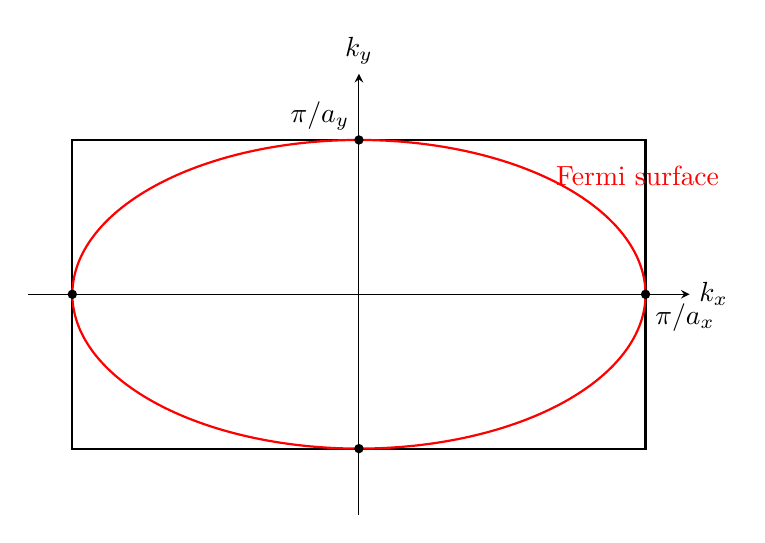
\begin{tikzpicture}[>=stealth, scale=1.4]
  \draw[->] (-3.0,0) -- (3.0,0) node[right] {$k_x$};
  \draw[->] (0,-2.0) -- (0,2.0) node[above] {$k_y$};
  \draw[thick] (-2.6,-1.4) rectangle (2.6,1.4);
  % Approximate distorted Fermi surface: ellipse-like through (\pm 2.6,0) and (0,\pm 1.4)
  \draw[thick, red, smooth, samples=120, domain=0:360] plot ({2.6*cos(\x)}, {1.4*sin(\x)});
  \node[circle,fill,inner sep=1.2pt] at ( 2.6,0) {};
  \node[circle,fill,inner sep=1.2pt] at (-2.6,0) {};
  \node[circle,fill,inner sep=1.2pt] at (0, 1.4) {};
  \node[circle,fill,inner sep=1.2pt] at (0,-1.4) {};
  \node[below right] at ( 2.6,0) {$\pi/a_x$};
  \node[above left]  at (0, 1.4) {$\pi/a_y$};
  \node[red, above right] at (1.7, 0.9) {Fermi surface};
\end{tikzpicture}
\end{center}

Nesting at $\bm Q=(\pi/a_x,\pi/a_y)$ is preserved, hence again $\mu(T)=\epsilon_0$.

\section*{Question 3 --- Phonons in lead}

\textbf{Problem.} Define phonon and Brillouin zone. From the Morse potential ($\xi=\SI{0.084}{nm},\,A=\SI{1600}{eV},\,B=\SI{40}{eV}$) compute the equilibrium bond length $a$, binding energy and harmonic spring constant $\kappa$. Compute the 1D sound velocity (Pb, $M=\SI{207}{g\,mol^{-1}}$). Estimate the thermal-expansion coefficient using cubic anharmonicity, and identify the validity ranges in $T$.

\subsection*{(a) Definitions}

Phonon: a quantised normal mode of lattice vibration carrying energy $\hbar\omega$ and crystal momentum $\hbar\bm k$, obeying Bose--Einstein statistics.

Brillouin zone: the Wigner--Seitz primitive cell of the reciprocal lattice; equivalently, the set of $\bm k$ closer to the origin than to any other reciprocal lattice point.

\subsection*{(b) Morse: $a$, $V_{\min}$, $\kappa$}

Set $u\equiv e^{-r/\xi}$:
\[
V = A u^2 - B u.
\]
Differentiate w.r.t.\ $r$ via $\de u/\de r = -u/\xi$:
\[
V'(r) = -\frac{u}{\xi}(2A u - B).
\]
Equilibrium $V'(a)=0$:
\[
u_a = \frac{B}{2A}.
\]
Invert $u_a = e^{-a/\xi}$:
\[
a = \xi\ln\frac{2A}{B}.
\]
Numerical: $2A/B = 80$, $\ln 80 = 4.382$:
\[
\boxed{\;a = \SI{0.084}{nm}\times 4.382 = \SI{0.368}{nm}.\;}
\]

Binding energy: insert $u_a=B/(2A)$ into $V$:
\[
V(a) = A\left(\frac{B}{2A}\right)^2 - B\cdot\frac{B}{2A} = \frac{B^2}{4A} - \frac{B^2}{2A}.
\]
Simplify:
\[
\boxed{\;V(a) = -\frac{B^2}{4A} = -\frac{(40)^2}{4\cdot 1600}\,\si{eV} = \SI{-0.250}{eV}.\;}
\]

Second derivative. Differentiate $V'(r) = -(u/\xi)(2Au-B)$ once more:
\[
V''(r) = \frac{1}{\xi^2}(4A u^2 - B u).
\]
Evaluate at $u=u_a$:
\[
\kappa \equiv V''(a) = \frac{1}{\xi^2}\left(4A\cdot\frac{B^2}{4A^2} - B\cdot\frac{B}{2A}\right) = \frac{B^2}{2A\xi^2}.
\]
Numerical (in eV per nm$^2$):
\[
\kappa = \frac{40^2}{2\cdot 1600\cdot(0.084)^2}\,\si{eV\,nm^{-2}} = 70.9\,\si{eV\,nm^{-2}}.
\]
Convert to SI: $1\,\si{eV\,nm^{-2}} = \SI{1.602e-19}{J}/\SI{e-18}{m^2} = \SI{0.1602}{N\,m^{-1}}$:
\[
\boxed{\;\kappa \approx \SI{11.4}{N\,m^{-1}}.\;}
\]

\subsection*{(c) Sound velocity}

Monatomic chain dispersion:
\[
\omega(k) = 2\sqrt{\kappa/m}\,|\sin(ka/2)|.
\]
Long-wavelength group velocity $v_s = \de\omega/\de k|_{k\to 0}$:
\[
v_s = a\sqrt{\kappa/m}.
\]
Atomic mass:
\[
m = \frac{M}{N_A} = \frac{\SI{0.207}{kg\,mol^{-1}}}{\SI{6.022e23}{mol^{-1}}} = \SI{3.44e-25}{kg}.
\]
Compute $\kappa/m$:
\[
\frac{\kappa}{m} = \frac{11.4}{3.44\times 10^{-25}}\,\si{s^{-2}} = \SI{3.31e25}{s^{-2}}.
\]
Square root:
\[
\sqrt{\kappa/m} = \SI{5.76e12}{s^{-1}}.
\]
Multiply by $a$:
\[
\boxed{\;v_s = (\SI{0.368e-9}{m})\times(\SI{5.76e12}{s^{-1}}) \approx \SI{2.1e3}{m\,s^{-1}}.\;}
\]
Compare measured Pb longitudinal speed $\sim\SI{2000}{m\,s^{-1}}$: agreement.

\subsection*{(d) Thermal expansion from cubic anharmonicity}

Expand $V$ to cubic order around $r=a$, with $x\equiv r-a$:
\[
V(r) \approx V(a) + \tfrac12\kappa\,x^2 + \tfrac16\kappa_3\,x^3,\qquad \kappa_3 \equiv V'''(a).
\]
Differentiate $V''$ once more:
\[
V'''(r) = -\frac{1}{\xi^3}(8A u^2 - B u).
\]
Insert $u_a=B/(2A)$:
\[
\kappa_3 = -\frac{1}{\xi^3}\left(\frac{2B^2}{A} - \frac{B^2}{2A}\right) = -\frac{3B^2}{2A\xi^3} < 0.
\]

Treat cubic term as perturbation; harmonic averages $\langle x\rangle_0 = 0$, $\langle x^2\rangle_0 = k_B T/\kappa$, $\langle x^3\rangle_0 = 0$, $\langle x^4\rangle_0 = 3(k_B T/\kappa)^2$.

First-order in $\kappa_3$:
\[
\langle x\rangle \approx -\frac{\kappa_3}{6 k_B T}\langle x^4\rangle_0.
\]
Substitute $\langle x^4\rangle_0$:
\[
\langle x\rangle = -\frac{\kappa_3}{6 k_B T}\cdot 3\left(\frac{k_B T}{\kappa}\right)^2 = -\frac{\kappa_3 k_B T}{2\kappa^2}.
\]
Differentiate w.r.t.\ $T$ and divide by $a$:
\[
\boxed{\;\alpha = \frac{1}{a}\frac{\de\langle r\rangle}{\de T} \sim \frac{|\kappa_3|\,k_B}{\kappa^2 a}.\;}
\]

Numerical sanity check: $|\kappa_3| = 3B^2/(2A\xi^3)$. Convert to SI: $\kappa_3 \sim \SI{4e-9}{J\,m^{-3}}$ (i.e.\ $\sim\SI{4e9}{N\,m^{-2}}$ in spring units). With $\kappa=\SI{11.4}{N\,m^{-1}}$, $a=\SI{0.368}{nm}$, $k_B = \SI{1.38e-23}{J\,K^{-1}}$:
\[
\alpha \sim \frac{(\SI{4e9}{N\,m^{-2}})(\SI{1.38e-23}{J\,K^{-1}})}{(\SI{11.4}{N\,m^{-1}})^2(\SI{3.68e-10}{m})} \sim \SI{e-4}{K^{-1}}.
\]
Order-of-magnitude correct (measured $\alpha_{\text{Pb}}\approx\SI{2.9e-5}{K^{-1}}$); positive sign because $\kappa_3<0$ widens the well asymmetrically outwards.

\subsection*{(e) Validity ranges}

\textbf{(i) Cubic-only expansion.} Require harmonic $\gg$ cubic energy scale, $\langle\tfrac12\kappa x^2\rangle\gg\langle\tfrac16|\kappa_3|x^3\rangle$ at thermal amplitude $|x|\sim\sqrt{k_B T/\kappa}$:
\[
\kappa \gg \frac{|\kappa_3|}{3}\sqrt{k_B T/\kappa}.
\]
Square and rearrange:
\[
k_B T \ll \frac{9\kappa^3}{\kappa_3^2}.
\]
Numerically this gives $T\ll\SI{e3}{K}$; the physical upper bound is set by the well depth $|V(a)|/k_B \approx \SI{2900}{K}$ (or in practice the lead melting point $T_m\approx\SI{600}{K}$):
\[
\boxed{\;T \lesssim T_m \approx \SI{600}{K}.\;}
\]

\textbf{(ii) Quantum mechanics important.} Compare $\hbar\omega$ to $k_B T$ with $\omega = \sqrt{\kappa/m} = \SI{5.76e12}{s^{-1}}$:
\[
T_Q \sim \frac{\hbar\omega}{k_B} = \frac{(\SI{1.055e-34}{J\,s})(\SI{5.76e12}{s^{-1}})}{\SI{1.381e-23}{J\,K^{-1}}}.
\]
Evaluate:
\[
\boxed{\;T_Q \approx \SI{40}{K}.\;}
\]
For $T\lesssim T_Q$ zero-point motion dominates ($\langle x^2\rangle\to\hbar/(2m\omega)$), heat capacity drops below $k_B$/mode (Debye/Einstein freeze-out), and $\alpha\propto T^3$ at low $T$ (Gr\"uneisen).

Classical cubic-only treatment is therefore valid in $T_Q \lesssim T \lesssim T_m$, i.e.\ roughly $\SI{40}{K}\lesssim T\lesssim\SI{600}{K}$.

\section*{Question 4 --- Magnetism of GdN}

\textbf{Problem.} Define paramagnet, diamagnet, ferromagnet (with examples). Find $S$ of $\mathrm{Gd}^{3+}$ ($4f^7$) by Hund. Treat $\mathrm{Gd}^{3+}$ as Ising along $\hat z$ in FCC GdN ($a=\SI{0.50}{nm}$): compute Curie constant $C$ for $\chi=C/T$, modify $\chi$ for $T>T_c=\SI{70}{K}$, give $M(T=0)$, and sketch $M(T)$ for $0\le T<2T_c$ at $H_z=0$ and $H_z>0$.

\subsection*{(a) Definitions}

Paramagnet: $\chi>0$, no spontaneous order; high-$T$ Curie law $\chi\propto 1/T$. Example: MnSO$_4$ (or any rare-earth salt above its ordering $T$).

Diamagnet: $\chi<0$, repelled from field, Larmor response of closed shells. Example: Cu, Bi, water.

Ferromagnet: spontaneous magnetisation $M\neq 0$ below Curie $T_c$. Example: Fe, Ni, Co.

\subsection*{(b) Spin of Gd$^{3+}$}

Configuration $4f^7$: half-filled shell. Hund's first rule maximises $S$, all 7 spins parallel:
\[
\boxed{\;S = 7/2.\;}
\]
(Hund 2: $L=0$; Hund 3: $J=S=7/2$, $g_J = 2$.)

\subsection*{(c) Curie constant}

Ising along $\hat z$ with $S=7/2$ and $g=2$: each ion is a two-level system with moment
\[
m = g\,S\,\mu_B = 2\cdot\tfrac72\,\mu_B = 7\mu_B.
\]
Energies $\mp m B$ in field $B=\mu_0 H_z$. Two-level partition function:
\[
Z = 2\cosh(\beta m B),\qquad \langle m_z\rangle = m\tanh(\beta m B).
\]
Linearise for $\beta m B\ll 1$:
\[
\langle m_z\rangle \approx \frac{m^2 B}{k_B T} = \frac{m^2 \mu_0 H_z}{k_B T}.
\]
Multiply by number density:
\[
M_z = n\langle m_z\rangle = \frac{n m^2 \mu_0}{k_B T} H_z.
\]
Read off:
\[
\chi = \frac{n m^2 \mu_0}{k_B T} = \frac{C}{T},\qquad C = \frac{n m^2 \mu_0}{k_B}.
\]

Number density: GdN is FCC with one formula unit per primitive cell, equivalently 4 Gd$^{3+}$ per conventional cell of side $a$:
\[
n = \frac{4}{a^3} = \frac{4}{(\SI{0.50e-9}{m})^3} = \SI{3.20e28}{m^{-3}}.
\]
Insert numbers (with $\mu_B = \SI{9.274e-24}{J\,T^{-1}}$, $\mu_0=4\pi\times\SI{e-7}{T\,m\,A^{-1}}$):
\[
C = \frac{(\SI{3.20e28}{m^{-3}})(7\cdot\SI{9.274e-24}{J\,T^{-1}})^2(4\pi\times\SI{e-7}{T\,m\,A^{-1}})}{\SI{1.381e-23}{J\,K^{-1}}}.
\]
Evaluate $(7\mu_B)^2 = (\SI{6.49e-23}{J\,T^{-1}})^2 = \SI{4.21e-45}{J^2\,T^{-2}}$:
\[
C = \frac{(\SI{3.20e28}{})(\SI{4.21e-45}{})(\SI{1.257e-6}{})}{\SI{1.381e-23}{}}\,\si{K}.
\]
Multiply numerator: $\SI{1.69e-22}{}$:
\[
\boxed{\;C \approx \SI{12.3}{K}.\;}
\]

\subsection*{(d) Curie--Weiss modification and $M(0)$}

Mean-field treatment of exchange: replace $T$ by $T-T_c$:
\[
\boxed{\;\chi(T) = \frac{C}{T - T_c}\quad\text{for }T > T_c.\;}
\]
Denominator vanishes at $T_c$, signalling spontaneous order.

At $T=0$ Ising spins fully align: $M(0) = n m$. Insert:
\[
M(0) = (\SI{3.20e28}{m^{-3}})\times 7\times(\SI{9.274e-24}{J\,T^{-1}}).
\]
Evaluate:
\[
\boxed{\;M(0) \approx \SI{2.1e6}{A\,m^{-1}}.\;}
\]

\subsection*{(e) $M(T)$ sketch}

\begin{center}
\begin{tikzpicture}[>=stealth, scale=1.2]
  \draw[->] (0,0) -- (8.5,0) node[right] {$T$};
  \draw[->] (0,0) -- (0,4.0) node[above] {$M(T)$};
  % Mark Tc and 2Tc
  \draw[dashed] (4,0) -- (4,3.4);
  \node[below] at (4,0) {$T_c$};
  \node[below] at (8,0) {$2T_c$};
  \node[circle,fill,inner sep=1.2pt] at (4,0) {};
  \node[circle,fill,inner sep=1.2pt] at (8,0) {};
  % H=0 curve: starts at M(0), drops to 0 at T_c with sqrt singularity, then 0
  \draw[thick, blue, smooth, samples=80, domain=0:3.99]
    plot ({\x}, {3.4*sqrt(1 - (\x/4)*(\x/4))});
  \draw[thick, blue] (4,0) -- (8.2,0);
  \node[circle,fill,inner sep=1.2pt] at (0,3.4) {};
  \node[left] at (0,3.4) {$M(0)$};
  \node[blue, above] at (1.4,3.2) {$H_z = 0$};
  % H>0 dashed curve: smooth crossover, never zero (split into two domains)
  \draw[thick, red, dashed, smooth, samples=80, domain=0:3.95]
    plot ({\x}, {3.5*sqrt(1 - (\x/4)*(\x/4))*0.95 + 0.6});
  \draw[thick, red, dashed, smooth, samples=80, domain=3.95:8.2]
    plot ({\x}, {2.0/(\x-4+1.0) + 0.05});
  \node[red, above right] at (5.6,1.2) {$H_z > 0$};
  \node[above right] at (4.1,2.0) {smooth, no kink};
  \node[below right] at (5.5,0.4) {Curie--Weiss tail $M = C H_z/(T-T_c)$};
\end{tikzpicture}
\end{center}

Differences:
\begin{itemize}
  \item $H_z=0$: spontaneous $M$ only for $T<T_c$; $M\propto(T_c-T)^{1/2}$ near $T_c$ in mean-field; identically zero for $T\ge T_c$.
  \item $H_z>0$: field selects the $+\hat z$ branch, giving $M>0$ everywhere; sharp kink at $T_c$ smeared into a crossover; above $T_c$ a Curie--Weiss tail $M = C H_z/(T-T_c)\to 0$ only as $T\to\infty$.
\end{itemize}

\end{document}
